\documentclass[letterpaper,10pt]{article}

% Packages for formatting
\usepackage{enumitem} % For customizing lists
\usepackage{array} % For customizing tables
\usepackage[empty]{fullpage}
\usepackage{titlesec}
\usepackage{graphicx}
\usepackage{enumitem}
\usepackage[hidelinks]{hyperref}
\usepackage{xcolor}
\usepackage{fontawesome}

% Page formatting
\pagestyle{empty}
\setlength{\parskip}{0.9em}

% Images Sourcing
\graphicspath{{public/img}}

% Section formatting
\titleformat{\section}{
  \vspace{-8pt}\scshape\raggedright\large
}{}{0em}{}[\color{black}\titlerule \vspace{-2pt}]

% Custom commands for bullets and date entry
\newcommand{\resumeItem}[1]{
  \item\small{
    {#1 \vspace{-2pt}}
  }
}

\newcommand{\resumeSubheading}[4]{
  \vspace{-1pt}
  \item
  \begin{tabular*}{0.97\textwidth}{l@{\extracolsep{\fill}}r}
    \textbf{#1} & #2 \\
    \textit{\small#3} & \textit{\small #4} \\
  \end{tabular*}\vspace{-5pt}
}

% Information Section
\begin{document}

\hypersetup{
    linkcolor=blue,
    urlcolor=blue,
    linkbordercolor=blue,
    citebordercolor=blue
}

\begin{center}
  {\huge\scshape Furqan Ramadhan} \\ \vspace{5pt}
  furqan2682@gmail.com $|$ 085207879445 $|$ Banda Aceh, Indonesia \\
  \vspace{5pt}
  \textit{Connect with me:} \\
  \href{https://www.linkedin.com/in/furqan-ramadhan-a86808179}{\color{blue}\faLinkedin}~linkedin.com/in/furqan-ramadhan-a86808179 \\
  \href{https://github.com/furqanramadhan}{\color{black}\faGithub}~github.com/furqanramadhan
\end{center}


\begin{figure}[h]
  \centering
  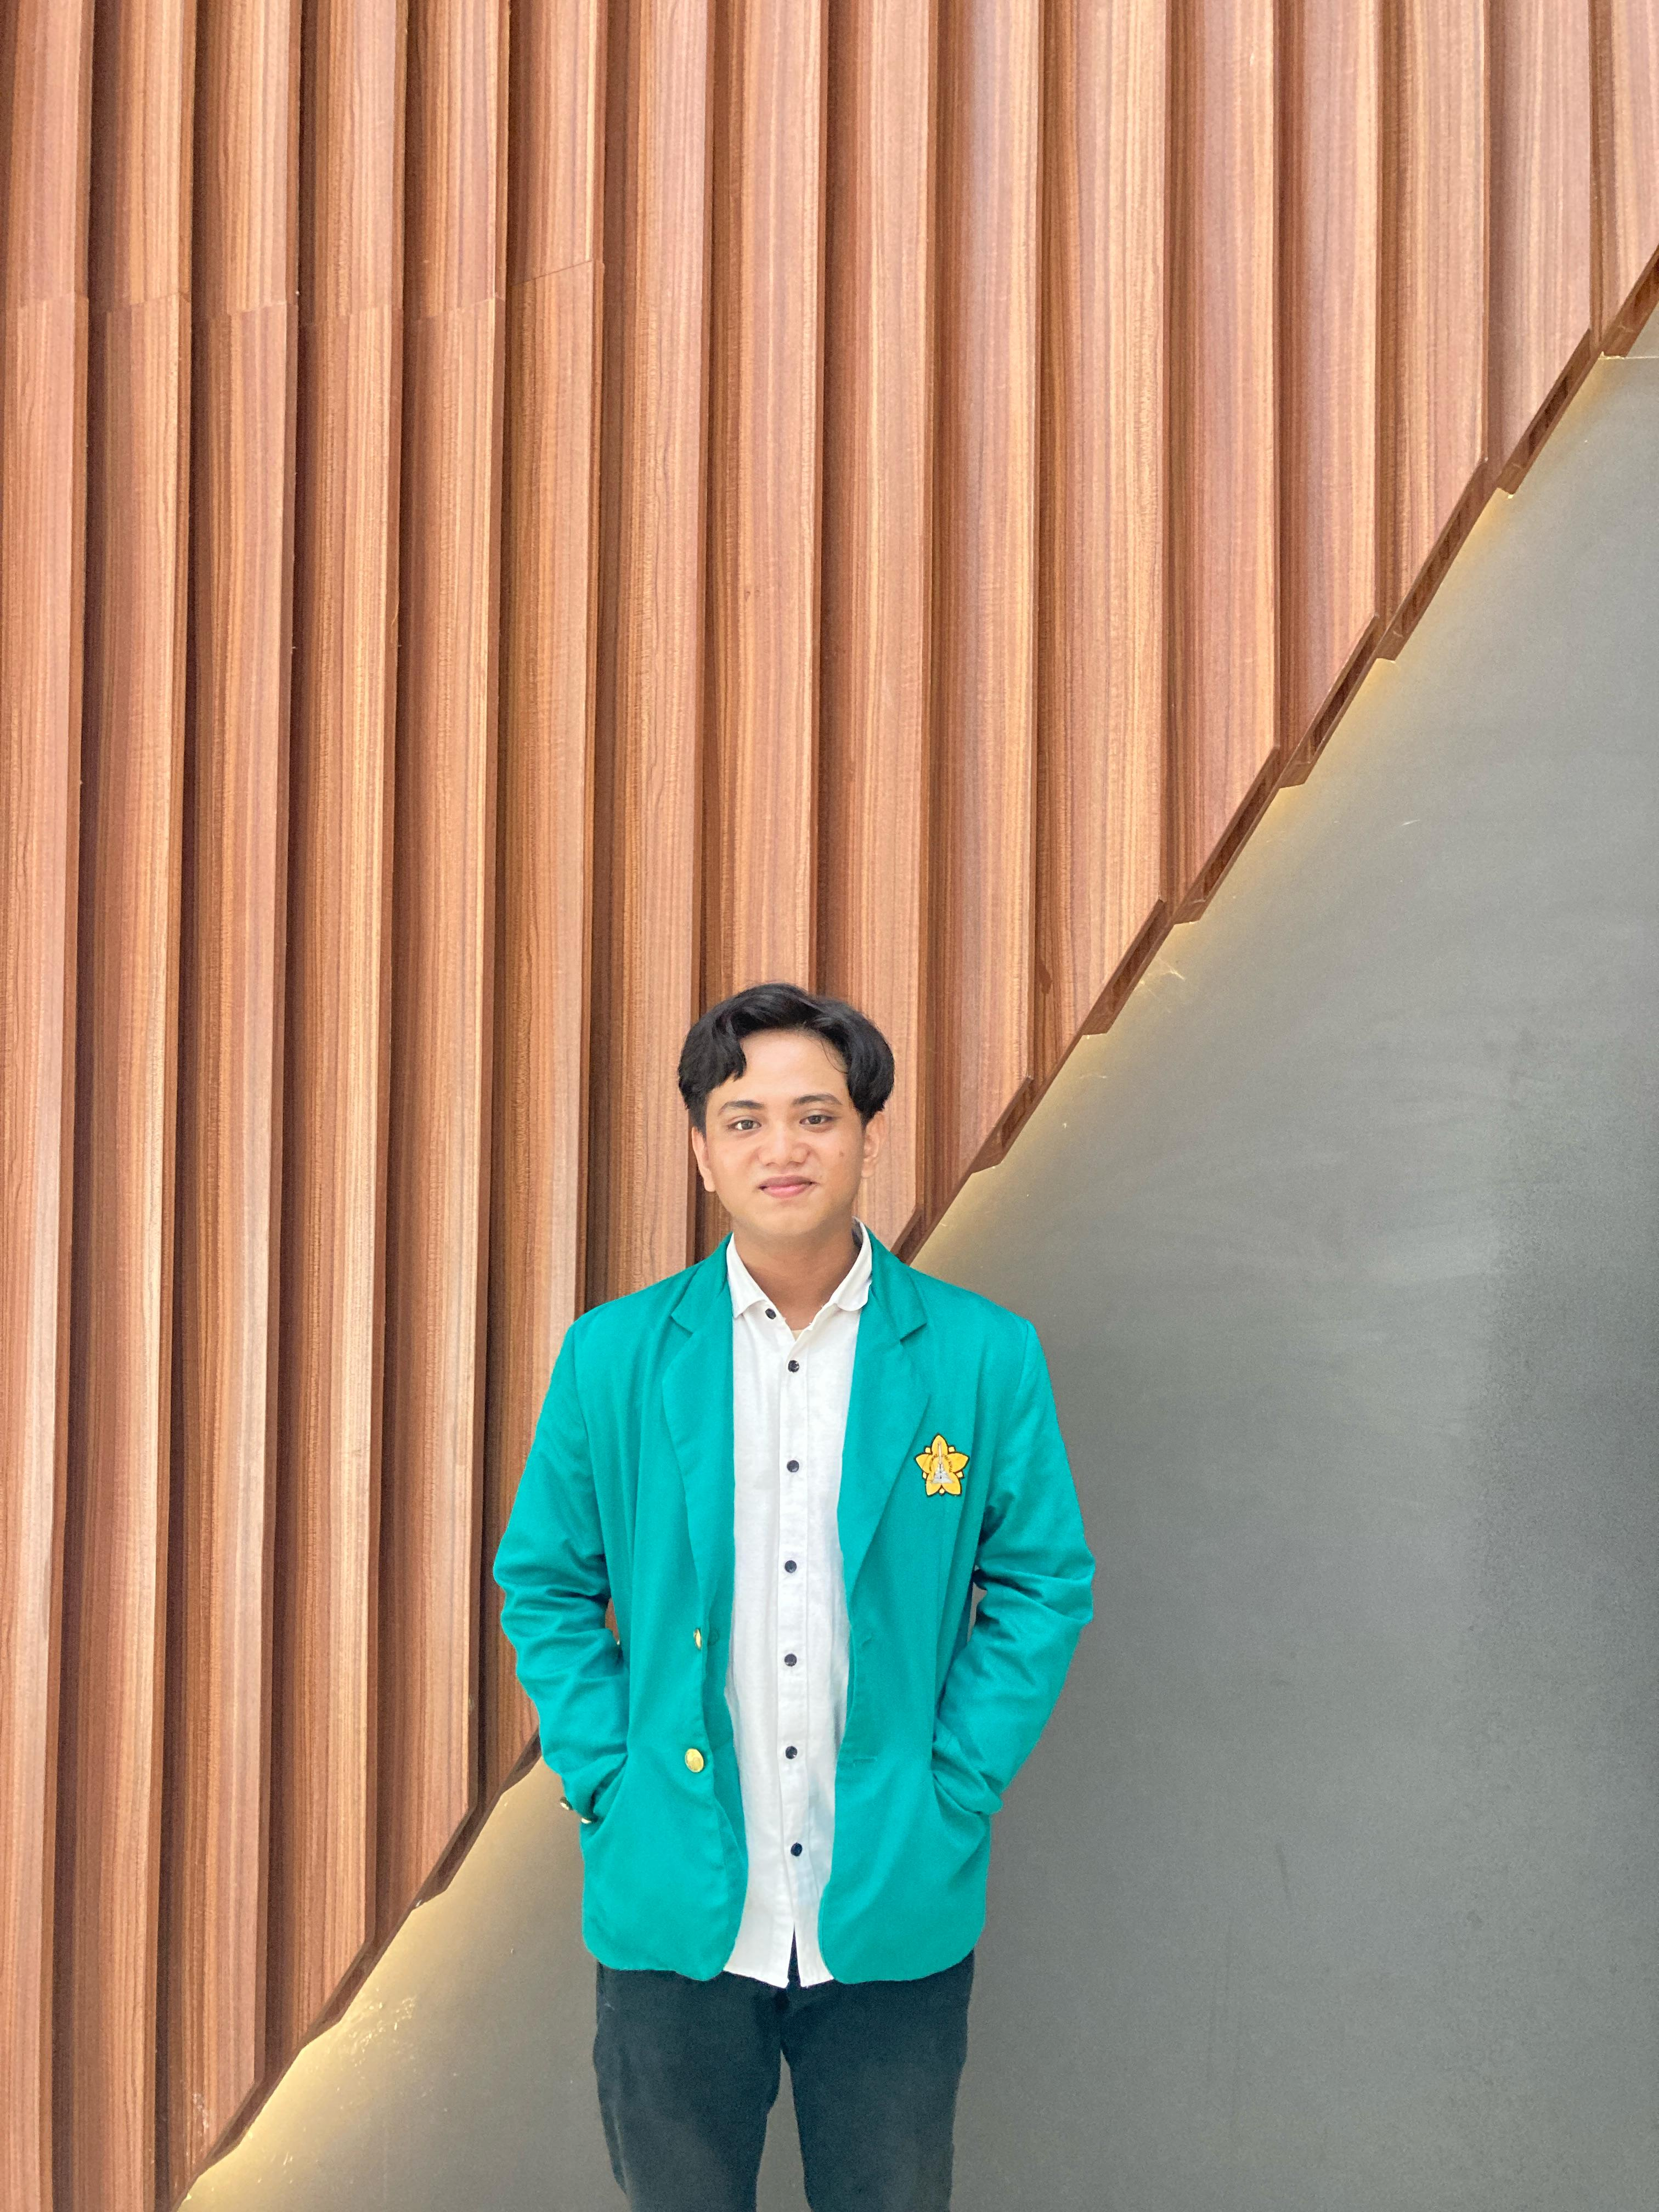
\includegraphics[width=6cm, height=8cm]{public/img/img_01.jpeg}
\end{figure}


% Summary Section
\section{Summary}

"A creative thinker who enjoys critical analysis, thrives at group ideation, and adeptly employs technology to establish inventive solutions. Rapid at embracing change and effectively to become proficient in cutting-edge IT disciplines."


% Experience Section
\section{Experience}
\begin{itemize}[leftmargin=0.15in, label={}]
  	\resumeSubheading{HMIF Website - Himpunan Mahasiswa Informatika}{In a team}{Frontend}{2024}
  	\resumeItem{Developing a Informatics Students Association as new our operational plan in this year. Using Next.js, Node.js Framework and JavaScript, implements UI/UX to website page which has been designed in a team. Hopefully will be completed in three months.}
	
    \resumeSubheading{Laboratory Assistant - Software Engineering}{Syiah Kuala University}{Laboratory Assistant}{2024}
    \resumeItem{Taught peers about basic AEIOU, Human Centered Design (HCD), functionality design, Unified Model Language (UML), and software engineering methodology using Agile Framework from basics to advanced topics, specifically with Scrum and Sprint Backlog.}
  \resumeSubheading{Web Based Pickup Service Coffee Ground Waste Request Application}{In a team}{Full Stack}{2023}
    \resumeItem{Developed an application in team to facilitate Service Coffee Waste to perform a pickup service sytem by Courier. Responsible for design UI and UX compliance using Figma. Build a robust database system, CRUD for Coffee Ground Waste, and also developed with Laravel framework.}
    \resumeSubheading{Capytype - Minimalistic Typing Test Web Based}{In a team}{Backend}{2023}
    \resumeItem{Developed web based application minimalistic typing test. Has an account system to user track users. Developed using the Laravel framework. Spearheaded for design an UX, implemented CRUD functionality for user accounts in the database. Devised JavaScript logic rule for the typing, ensuring seamless functionality of the website.}
    \resumeSubheading{Laboratory Assistant - Computer Network}{Syiah Kuala University}{Laboratory Assistant}{2023}
    \resumeItem{Taught peers about basic Netacad Cisco technology from basics to advanced topics such as introduction, installation, Protocol, IPv4/IPv6 Subnetting, Transport Layer and Application Layer, and also introduction to build a network in campus area.}
\end{itemize}

% Skills Section
\section{Skills}
  \begin{itemize}[leftmargin=0.15in, label={}]
    \item \textbf{Proficient in Linux : }{Regularly utilize Linux as the primary operating system}
    \item \textbf{C/C++: }{Skilled in problem-solving using C/C++.}
    \item \textbf{Object-Oriented Programming (OOP) : }{Thorough understanding of OOP concepts.}
    \item \textbf{MySQL/MariaDB : }{Frequently used and favored database systems.}
    \item \textbf{Web Development Frameworks : }{PHP (Laravel), Node.js, Express.js, Next.js}
    \item \textbf{Proficiency in HTML, CSS (Tailwind) : }{In-depth understanding of HTML and logical design in web development.}
    \item \textbf{Python (Pandas) : }{Regular usage for data processing and visualization.}
    \item \textbf{ChatGPT/Bard Prompt : }{Experience in using and interacting with ChatGPT or Bard for development.}
  \end{itemize}

% Organizational Involvement Section
\section{Social and Organizational Involvement}
\begin{itemize}[leftmargin=0.15in, label={}]
    \resumeSubheading{Pertukaran Mahasiswa Merdeka}{2023} {Provided by Ministry of Education, Culture, Research, and Technology.}{Institut Teknologi Nasional, Bandung}
    \resumeSubheading{Informatics Student Organization}{2023, 2024} {Informatics Student Organization at Syiah Kuala University,}{Banda Aceh, Indonesia}
    \resumeSubheading{Student Executive Board, Science and Math Faculty}{2022} {Under the guidance of the Faculty of Mathematics and Natural Sciences}{Banda Aceh, Indonesia}


    \begin{itemize}[leftmargin=0.07in, label={}]
      \item \textbf{Chairperson for Mangrove Plantation Committee - Student Executive Board, Science and Math Faculty Event 2022:} Oversaw and coordinated the event, collaborating with team members, ensuring meticulous planning to guarantee the successful execution of the mangrove plantation initiative.

      \item \textbf{Competitive Member - 'Infest' Event 2022:} Served as a member Infest (Informatics Event) of the Esports Pubg Mobile, actively participating in organizing and conducting events about techniques and rundown preparation. Collaborated with a team which experts in Pubg Mobile.
    \end{itemize}
\end{itemize}

% Education Section
\section{Education}
\vspace{-0.1in}  % Atur jarak vertikal di sini
\begin{itemize}[leftmargin=0.15in, label={}]
  \item \resumeSubheading{Informatics Undergraduate, Syiah Kuala University}{Expected Graduation: 2025}{GPA: 3.63}{Banda Aceh, Indonesia}
  \item \resumeSubheading{SMA Negeri 4 Banda Aceh}{Graduated: 2021}{High school interest in Science}{Banda Aceh, Indonesia}
\end{itemize}


% Hobbies & Interests Section
\section{Hobbies and Interests}
\begin{itemize}[leftmargin=0.15in, label={}]
    \item \textbf{Coding:}
        Enjoys learning new things through coding.

    \item \textbf{Learning History:}
        Usually learning from Youtube about another Country like Russia, Turkiye, Germany, and World War.
    
    \item \textbf{Hiking:}
        Was began during an independent student exchange (Pertukaran Mahasiswa Merdeka) with friends who had experience in mountainous terrain.

    \item \textbf{Running/Workout :}
        Regularly engages in cardio activities or workout in gym to stay fit and healthy.

    \item \textbf{Playing Games:}
        Likes playing Mobile games or PC games in free time.
  \end{itemize}


\end{document}